\section{eo\-Dyn\-SGATransform$<$ EOT $>$ Class Template Reference}
\label{classeo_dyn_s_g_a_transform}\index{eoDynSGATransform@{eoDynSGATransform}}
eo\-Dyn\-SGATransform: transforms a population using genetic operators.  


{\tt \#include $<$eo\-SGATransform.h$>$}

Inheritance diagram for eo\-Dyn\-SGATransform$<$ EOT $>$::\begin{figure}[H]
\begin{center}
\leavevmode
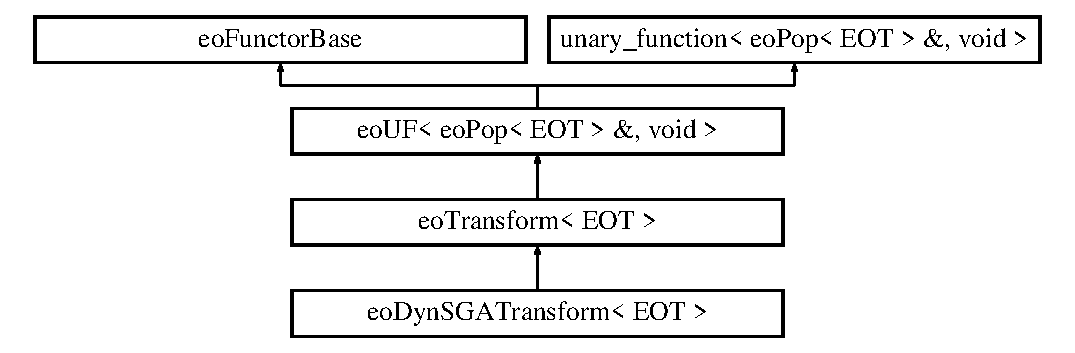
\includegraphics[height=4cm]{classeo_dyn_s_g_a_transform}
\end{center}
\end{figure}
\subsection*{Public Member Functions}
\begin{CompactItemize}
\item 
{\bf eo\-Dyn\-SGATransform} ({\bf eo\-Quad\-Op}$<$ {\bf EOT} $>$ \&\_\-cross, double \_\-c\-Proba, {\bf eo\-Mon\-Op}$<$ {\bf EOT} $>$ \&\_\-mutate, double \_\-m\-Proba)\label{classeo_dyn_s_g_a_transform_a0}

\begin{CompactList}\small\item\em Default constructor - receives values. \item\end{CompactList}\item 
{\bf eo\-Dyn\-SGATransform} ({\bf eo\-Quad\-Op}$<$ {\bf EOT} $>$ \&\_\-cross, double $\ast$\_\-c\-Proba\-Ref, {\bf eo\-Mon\-Op}$<$ {\bf EOT} $>$ \&\_\-mutate, double $\ast$\_\-m\-Proba\-Ref)\label{classeo_dyn_s_g_a_transform_a1}

\begin{CompactList}\small\item\em This constructor receives pointers. \item\end{CompactList}\item 
void {\bf operator()} ({\bf eo\-Pop}$<$ {\bf EOT} $>$ \&\_\-pop)
\begin{CompactList}\small\item\em Transforms a population. \item\end{CompactList}\item 
double \& {\bf PCross\-Handle} ()\label{classeo_dyn_s_g_a_transform_a3}

\item 
double \& {\bf PMut\-Handle} ()\label{classeo_dyn_s_g_a_transform_a4}

\end{CompactItemize}
\subsection*{Private Attributes}
\begin{CompactItemize}
\item 
{\bf eo\-Invalidate\-Quad\-Op}$<$ {\bf EOT} $>$ {\bf cross}\label{classeo_dyn_s_g_a_transform_r0}

\item 
double {\bf crossover\-Proba\-Holder}\label{classeo_dyn_s_g_a_transform_r1}

\item 
double \& {\bf crossover\-Proba}\label{classeo_dyn_s_g_a_transform_r2}

\item 
{\bf eo\-Invalidate\-Mon\-Op}$<$ {\bf EOT} $>$ {\bf mutate}\label{classeo_dyn_s_g_a_transform_r3}

\item 
double {\bf mutation\-Proba\-Holder}\label{classeo_dyn_s_g_a_transform_r4}

\item 
double \& {\bf mutation\-Proba}\label{classeo_dyn_s_g_a_transform_r5}

\end{CompactItemize}


\subsection{Detailed Description}
\subsubsection*{template$<$class EOT$>$ class eo\-Dyn\-SGATransform$<$ EOT $>$}

eo\-Dyn\-SGATransform: transforms a population using genetic operators. 

It is the Dynamic version of the above {\bf eo\-SGATransform}{\rm (p.\,\pageref{classeo_s_g_a_transform})} i.e. the operators probabilities can be passed as an {\bf eo\-Value\-Param}{\rm (p.\,\pageref{classeo_value_param})}, and hence can be modified from outside It is here mainly for tutorial reasons 



Definition at line 98 of file eo\-SGATransform.h.

\subsection{Member Function Documentation}
\index{eoDynSGATransform@{eo\-Dyn\-SGATransform}!operator()@{operator()}}
\index{operator()@{operator()}!eoDynSGATransform@{eo\-Dyn\-SGATransform}}
\subsubsection{\setlength{\rightskip}{0pt plus 5cm}template$<$class EOT$>$ void {\bf eo\-Dyn\-SGATransform}$<$ {\bf EOT} $>$::operator() ({\bf eo\-Pop}$<$ {\bf EOT} $>$ \& {\em \_\-pop})\hspace{0.3cm}{\tt  [inline, virtual]}}\label{classeo_dyn_s_g_a_transform_a2}


Transforms a population. 

\begin{Desc}
\item[Parameters:]
\begin{description}
\item[{\em pop}]The population to be transformed. \end{description}
\end{Desc}


Implements {\bf eo\-UF$<$ eo\-Pop$<$ EOT $>$ \&, void $>$} {\rm (p.\,\pageref{classeo_u_f_a1})}.

Definition at line 125 of file eo\-SGATransform.h.

References eo\-Rng::flip().

The documentation for this class was generated from the following file:\begin{CompactItemize}
\item 
eo\-SGATransform.h\end{CompactItemize}
